
\section{Rodzaje fal sprężystych}
\label{sec:rodzaje_fal_sprezystych}

Fale można podzielić ze względu na sposób w jaki propagują w materiale. Mogą to być fale podłużne lub poprzeczne. Fale takie propagują jeśli długość fali jest mniejsza lub bliska wymiarom ośrodka. Fale o długości przekraczającej wyraźnie przynajmniej jeden z wymiarów falowodu nazywamy falami prowadzonymi i mają one zupełnie inne własności. W takim przypadku występują dodatkowe rodzaje fal jak fale Rayleigha czy Lamba. Fala Rayleigha propagują na powierzchniach, stąd ośrodek musi być ograniczony przynajmniej jedną płaszczyzną. Fale Lamba propagują na strukturach cienkościennych.

\subsection{Fale podłużne}

Fale podłużne to fale, w których kierunek propagacji jest równoległy z kierunkiem drgania cząstek. Tego typu fale mogą rozchodzić się w każdym ośrodku materialnym. Przykładem fali podłużnej jest fala dźwiękowa rozchodząca się w powietrzu, pokazana na rysunku \ref{fig:fala_podluzna}. Prędkoś fali podłużnej w nieograniczonym ośrodku zależy od parametrów materiałowych ośrodka i dana jest wzorem:

\begin{equation}
c_L=\sqrt{\frac{\lambda+2\mu}{\rho}}
\end{equation}
gdzie
\begin{eqwhere}[2cm]
        \item[$c_L$] prędkość fali podłużnej
        \item[$\lambda, \mu$] stałe Lam\'{e}go
        \item[$\rho$] gęstość ośrodka
\end{eqwhere}

\begin{figure}[h]
\centering
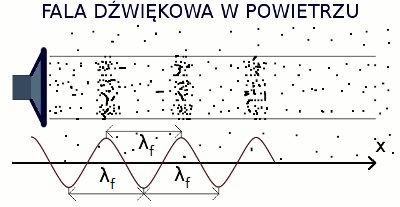
\includegraphics[width=10cm]{Zdjecia/2/fala_podluzna}
\caption{Przykład fali podłużnej}
\label{fig:fala_podluzna}
\end{figure}

Długością fali \( \lambda_f \) nazywamy odległoś między dwoma maksimami (lub minimami), które oznaczają maksymalne zagęszczenie (rozrzedzenie) cząstek w materiale.

\subsection{Fale poprzeczne}

Fale poprzeczne propagują w kierunku prostopadłum do kierunku drgań cząstek. Przykładami takich fal są fale elektromagnetyczne, fale propagacji naprężeń w materiale stałym, czy fala na zamocowanym jednostronnie sznurze, pokazana na rysunku \ref{fig:fala_poprzeczna}. Prędkoś fali poprzecznej w nieograniczonym ośrodku wyraża się wzorem:

\begin{equation}
c_T=\sqrt{\frac{\mu}{\rho}}
\end{equation}
gdzie
\begin{eqwhere}[2cm]
        \item[$c_T$] prędkość fali poprzecznej
        \item[$\mu$] stała Lam\'{e}go
        \item[$\rho$] gęstość ośrodka
\end{eqwhere}

\begin{figure}[h]
\centering
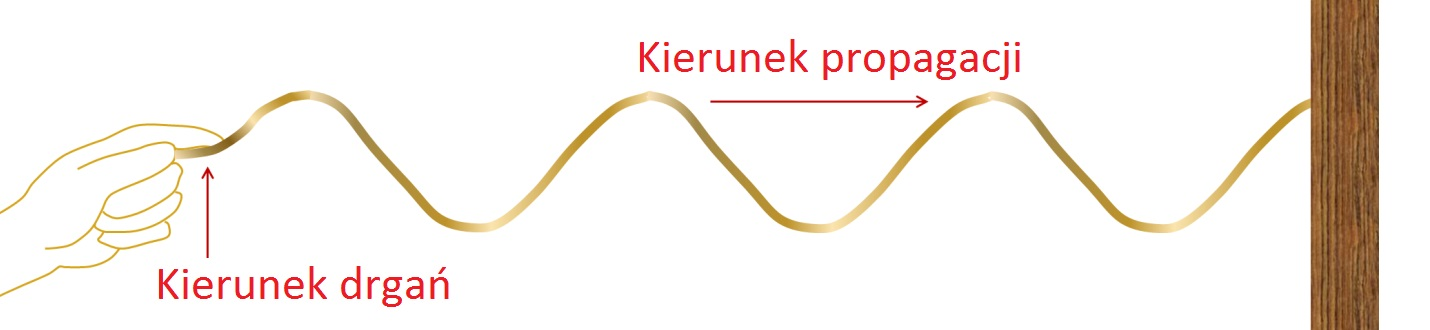
\includegraphics[width=10cm]{Zdjecia/2/fala_poprzeczna}
\caption{Przykład fali poprzecznej}
\label{fig:fala_poprzeczna}
\end{figure}

\subsection{Fale Rayleigha i L\"{o}va}

Opisane wcześniej fale propagują w nieograniczonych mediach. Fale Rayleigha oraz L\"{o}va są falami propagującymi w obszarze powierzchni ciał stałych. Dla fal Rayleigha drgania cząstek odbywają się równolegle oraz prostopadle do kierunku rozchodzenia się fali, zataczając elipsy. Kierunek prostopadły jest normalny do płaszczyzny, na której fala propaguje. Prędkoś fal Rayleigha dla metalu można wyrazić za pomocą współczynnik Poissona i prędkości fal poprzecznych:

\begin{equation}
c_R=\frac{0.87+1.12\cdot\nu}{1+\nu}\cdot c_T
\end{equation}
gdzie
\begin{eqwhere}[2cm]
        \item[$c_R$] prędkość fali Rayleigha
        \item[$c_T$] prędkość fali poprzecznej
        \item[$\nu$] współczynnik Poissona
\end{eqwhere}

Fale L\"{o}va to fale, w których drgania zachodzą w kierunku prostopadłym do kierunku, ale równolegle do płaszczyzny propagacji. Takie fale są wykorzystywane przy badaniu układów wielowarstwowych. Są silnie dyspersyjne, co oznacza że ich prędkość jest funkcją częstotliwości. Fala Rayleigha i L\"{o}va są zilustrowane na rysunku \ref{fig:fale_pow}.

\begin{figure}[h]
        \centering
        \begin{subfigure}{0.35\textwidth}
                \centering
	     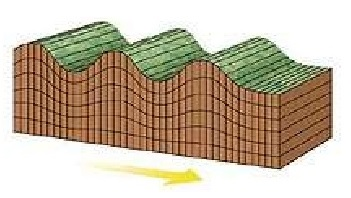
\includegraphics[width=5cm]{Zdjecia/2/fala_rayleigha}
                \subcaption{\label{subfigure_a}}
        \end{subfigure}
        \begin{subfigure}{0.35\textwidth}
                \centering
	     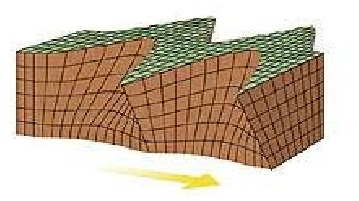
\includegraphics[width=5cm]{Zdjecia/2/fala_lova}
                \subcaption{\label{subfigure_b}}
        \end{subfigure}
        \label{fig:fale_pow}
        \caption{Fale powierzchniowe: \protect\subref{subfigure_a} fala Rayleigha, \protect\subref{subfigure_b} fala L\"{o}va}
\end{figure}

\subsection{Fale Lamba}

Ważnym typem fal, z racji na szerokie zastosowanie, są fale Lamba. Propagują one na cienkościennych elementach jak płyty, czy rury. Tego typu fale powstają na skutek złożenia dwóch fal Rayleigha, propagujących na płaszczyznach po obu stronach obiektu. Fale Lamba można podzielić na fale symetryczne, kiedy obie fale składowe propagują w tej samej fazie i asntysymetryczne kiedy propagują w przeciwnych fazach. Prędkość fal Lamba zależna jest od częstotliwości, ze względu na dyspersyjny charakter. Rysunek \ref{fig:fala_lamba} przedstawia podstaci fal Lamba.

\begin{figure}[h]
\centering
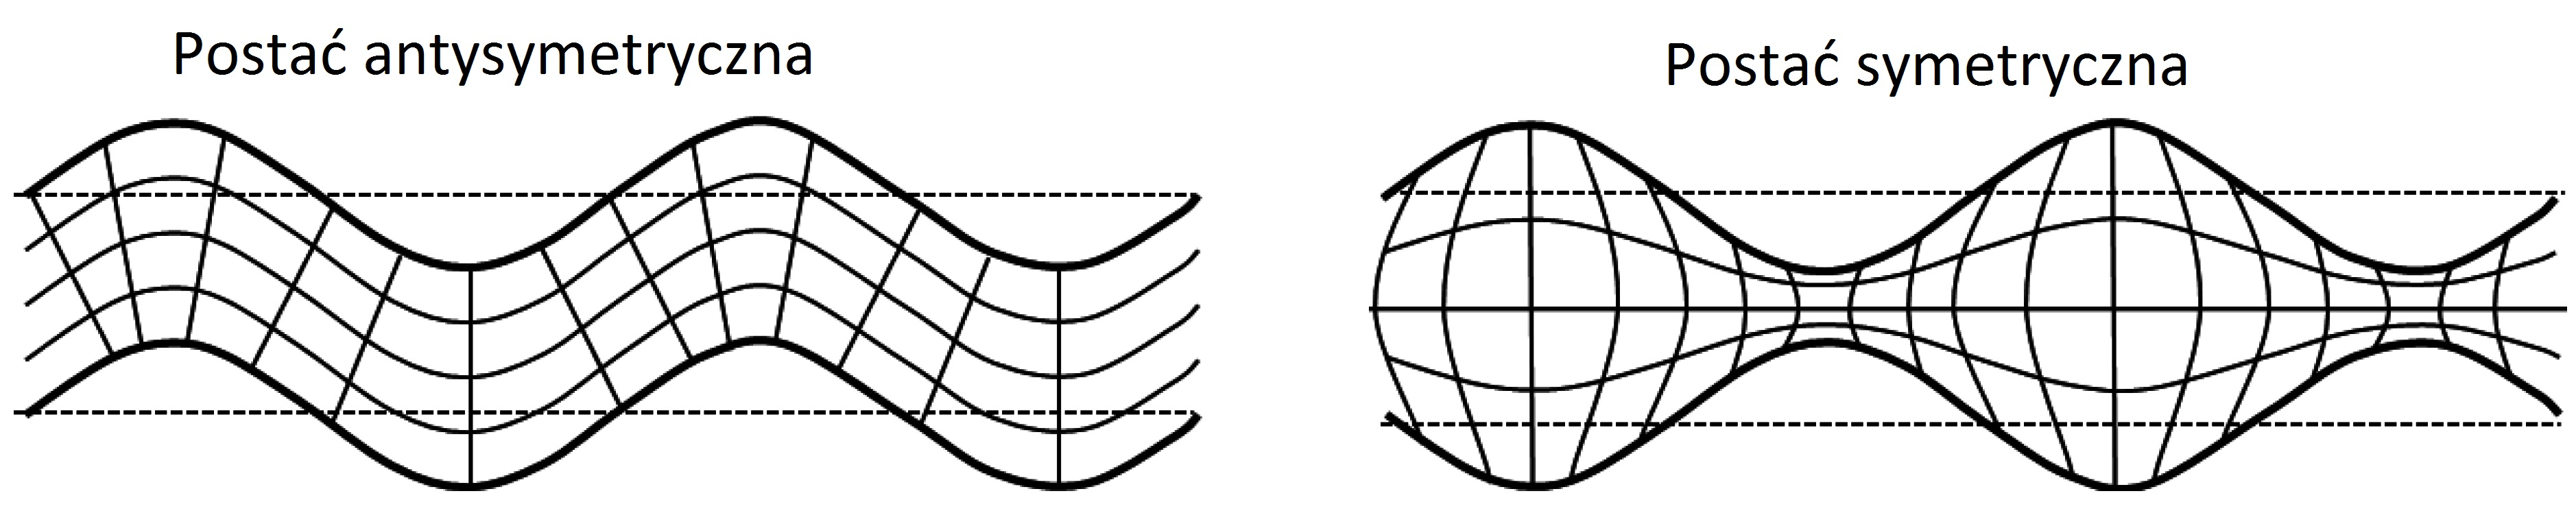
\includegraphics[width=14cm]{Zdjecia/2/fala_lamba}
\caption{Fale Lamba}
\label{fig:fala_lamba}
\end{figure}

%---------------------------------------------------------------------------





















